% !TEX root = ../main.tex
\chapter{Employ the Learned Deep Model}\label{ch:chapter5} % For referencing the chapter elsewhere, use \ref{Chapter1}
%
%%----------------------------------------------------------------------------------------
%
After we have obtained the learned models 
which exhibit desired behaviors, 
their integration into the reference software is carried out.
In this chapter, the time cost of the model prediction
is analyzed and optimizing methods are described.
After that we explain the details of the algorithm for integration.
Lastly the results of experiments 
are presented with discussions.

\section{Analysis and Optimization for Prediction Time}\label{sec:analysis-and-optimization}
% In C++ APIs from Tensorflow version 1.1, if we want to run the prediction,
% a unique session has to be initialized in which the predicting activities 
% take place.
% It is found that the session initialization is very time expensive.
It is intuitive to think in this way: 
every time when the encoder encounters a new block in the video frames,
the learned models are required to perform the prediction for that block.
However, after this idea has been implemented, it turns out the
time cost of the encoder with neural engine even gets much higher 
than the encoder without neural engine.
We found that the idea of one prediction for one block actually
introduces a problem that impedes the integration to work as expected:
a new session is initialized for a prediction, and the initialization
for a single session in Tensorflow C++ APIs is really time
expensive.
The other idea which is a better way would be a single 
session for a batch of blocks.

The time cost of session initialization has been investigated
and compared between the two ideas aforementioned.
The learned model for blocks of size \(8\times8\) is loaded 
to run predictions for blocks of size \(8\times8\) from one single
frame in one video sequence with the resolution to 
be \(1024\times768\).
Totally 12288 blocks to predict.
When compiling the executable binary of the encoder
powered by neural engine, it can be compiled 
against CPU or GPU when the compilation tool 
called Bazel~\parencite{RN200} is utilized.
Even more, with Bazel, the AVX and SSE4.2 can be employed to
accelerate the parallel computations in one instruction
at single moment in CPU\@.
They offer more efficient matrix computations
to CPU\@.
Six experiments have been conducted and the results
are shown in 
Table~\ref{tab:seesion-init-plain-cpu}.
% on page~\pageref{tab:seesion-init-plain-cpu}.

\begin{table}
    \caption{Time cost of session initialization for two ideas based on three sets of compiling configurations}
    \bigskip\label{tab:seesion-init-plain-cpu}
    \centering
    \begin{tabular}{c c c c c}
        \toprule
        \# & Idea & Plain CPU & AVX,SSE4.2 & AVX,SSE4.2,GPU \\
        \midrule
        1 & init 1 session for 12288 blocks & 21.37s &15.56s&2.03s \\
        2 & init 12288 sessions for 12288 blocks & 47.81s &33.91s&55.26s\\
        \bottomrule
    \end{tabular}
\end{table}

Obviously the best way is to compile the 
executable binary against AVX, SSE4.2 and GPU, at the same
time use the idea of one session for multiple blocks.

\section{The Integration of the Learned Model}\label{sec:integration-of-learned-model}
We have integrated two learned models into 
\(HTM16.2\) which is the newest version of
the reference software of 3D-HEVC by the time this thesis
is written\@.
More specifically, ResNet engines have been integrated to 
\textbf{\textit{TAppEncoder}} in \(HTM16.2\) for depth map 
angular modes [2, 34] prediction and the DMM1 searching process.
Wedgelet slope is employed
to reduce the number of wedgelet candidates to be evaluated in DMM1 
searching process. 
Since top-15 is used, roughly half of the candidates are skipped
during the encoding time.
The details of the proposed fast depth coding algorithm is shown 
in Figure~\ref{fig:proposed-fast-depth-coding-algorithm}
on page~\pageref{fig:proposed-fast-depth-coding-algorithm}.

Initially, before the encoding of a depth map will start, 
its Luma pixel values are accessed by the learned models to
predict best modes for all the suitable blocks inside it.
We call it \textbf{Batch Prediction}.
The model learned from blocks of size \(8\times8\) is used 
to predict the best modes for blocks of size \(8\times8\)
while the model learned from blocks of size \(16\times16\)
is used to predict the best modes for blocks of 
size \(16\times16\) and size \(32\times32\).
For example, in a video of resolution 
\(1024\times768\), each depth frame contains \(12,288\)
blocks of size \(8\times8\), \(3,072\) blocks of
size \(16\times16\) and \(768\) blocks of size 
\(32\times32\).
During depth map encoding, the learned models perform
predictions for all the \(12,288\)
blocks of size \(8\times8\), \(3,072\) blocks of
size \(16\times16\) and \(768\) blocks of size 
\(32\times32\).
The prediction results are stored in a map with 
three elements comprising size of block, CU position \(x\),
and CU position \(y\) as the key, 
and best mode as the value.
The information in this map will be retrieved 
using key to get the corresponding value
when recursively encoding CUs in 
this depth map.
For instance, given that the map is name as \(Map\),
the CU size is \(8\times8\) and CU position is \([x_c, y_c]\),
we can retrieve the best mode of this 
CU by \(BestMode_c = Map[8, x_c, y_c]\).
This map will be re-initialized to an empty map
every time a new depth frame will appear in the encoding.
Why is the implementation predicting best modes for all 
the \(12,288\) blocks of size \(8\times8\), 
\(3,072\) blocks of size \(16\times16\) and 
\(768\) blocks of size \(32\times32\)
when the depth frame will be encoded instead
of predicting best mode for
each CU when the CU will be encoded?
The first reason is, as shown in Section~\ref{sec:analysis-and-optimization},
the time cost is not acceptable if the prediction
is performed for each CU instead of for the whole
frame at each time.
The other reason is that when a depth frame will be
encoded, the CU partition information is 
not known to the encoder.
For this reason, it is necessary to perform 
predictions for all the possible CU candidates
to ensure that no matter how the CU partition scheme
will be, the information stored in the map
will be sufficient to help with the encoding.

Next, for each depth block of 
size \(8\times8\), \(16\times16\) and \(32\times32\), 
top-15 modes together with PLANAR, DC modes are added to 
a candidate list for Rough Mode Decision (RMD).
For blocks of other sizes, the original encoder workflow
is applied.
If mode 2 is inside the RMD List, mode 34
will be added to RMD List due to the reason that
it is of the same angle as mode 2.
Else if mode 2 is not inside the RMD List, 
mode 34 will not be added to RMD List.
The top-15 modes here is constructed by making reference to
the top-1 mode.
For example, if the top-1 mode is mode 10, 
the adjacent 14 modes will be added to the list of top-15.
Hence the list of modes will be 
[3, 4, 5, 6, 7, 8, 9, 10, 11, 12, 13, 14, 15, 16, 17].
After that, PLANAR and DC modes will be added to the list
of modes to form RMD List.
In our case, mode 33 and 
mode 2 are considered to be adjacent to each other.
Therefore, if the top-1 mode is mode 2, 
the list of modes will be
[9, 8, 7, 6, 5, 4, 3, 2, 33, 30, 29, 28, 27, 26, 25].
After that, mode 34, PLANAR and DC modes 
will be added to RMD List.
This method is based on the observations that 
the top-k predictions in confusion matrix
will always be the adjacent ones.

Then Sum of Absolute Transform Difference (SATD)
is used to obtain the best 3 candidates for blocks
of size \(8\times8\) and \(16\times16\), 2 candidates
for blocks of size \(32\times32\).
The number of candidates to be evaluated further 
is reduced for blocks of different types
comparing with the original implementation,
where 8 candidates will be selected for 
blocks of size \(8\times8\) and \(16\times16\), 
3 candidates will be selected
for blocks of size \(32\times32\).
The decision of candidates reduction in this step 
is due to the consideration that 
the model prediction has already narrowed
the searching range for mode candidates 
with a high precision such that
there is no need to evaluate
a large number of candidates in the
further steps.

After SATD, the best prediction of the block
is utilized to construct a range of slopes.
Denote the index of the top-1 mode from the model 
prediction as \(N_1\), a slope range will be constructed 
using the angular modes within \([N_1-7, N_1+7]\), where
the two boundaries are inclusive.
In the further step, when performing the DMM1 coarse
searching, the wedgelets which have the slopes out of the 
constructed slope range are excluded from 
View Synthesis Optimization (VSO) which is the
source of the computational complexity in the original
encoder.
The DMM1 refinement following the coarse search is unmodified.
In the end, the best mode for the
depth map to be coded in the encoding process will
be obtained.
This algorithm can reduce the number of wedgelet candidate by 
half.
Besides, the conventional intra 
angular mode decision for depth maps is also
accelerated using the same prediction from 
neural networks.
% First 

\begin{figure}
    \centering
    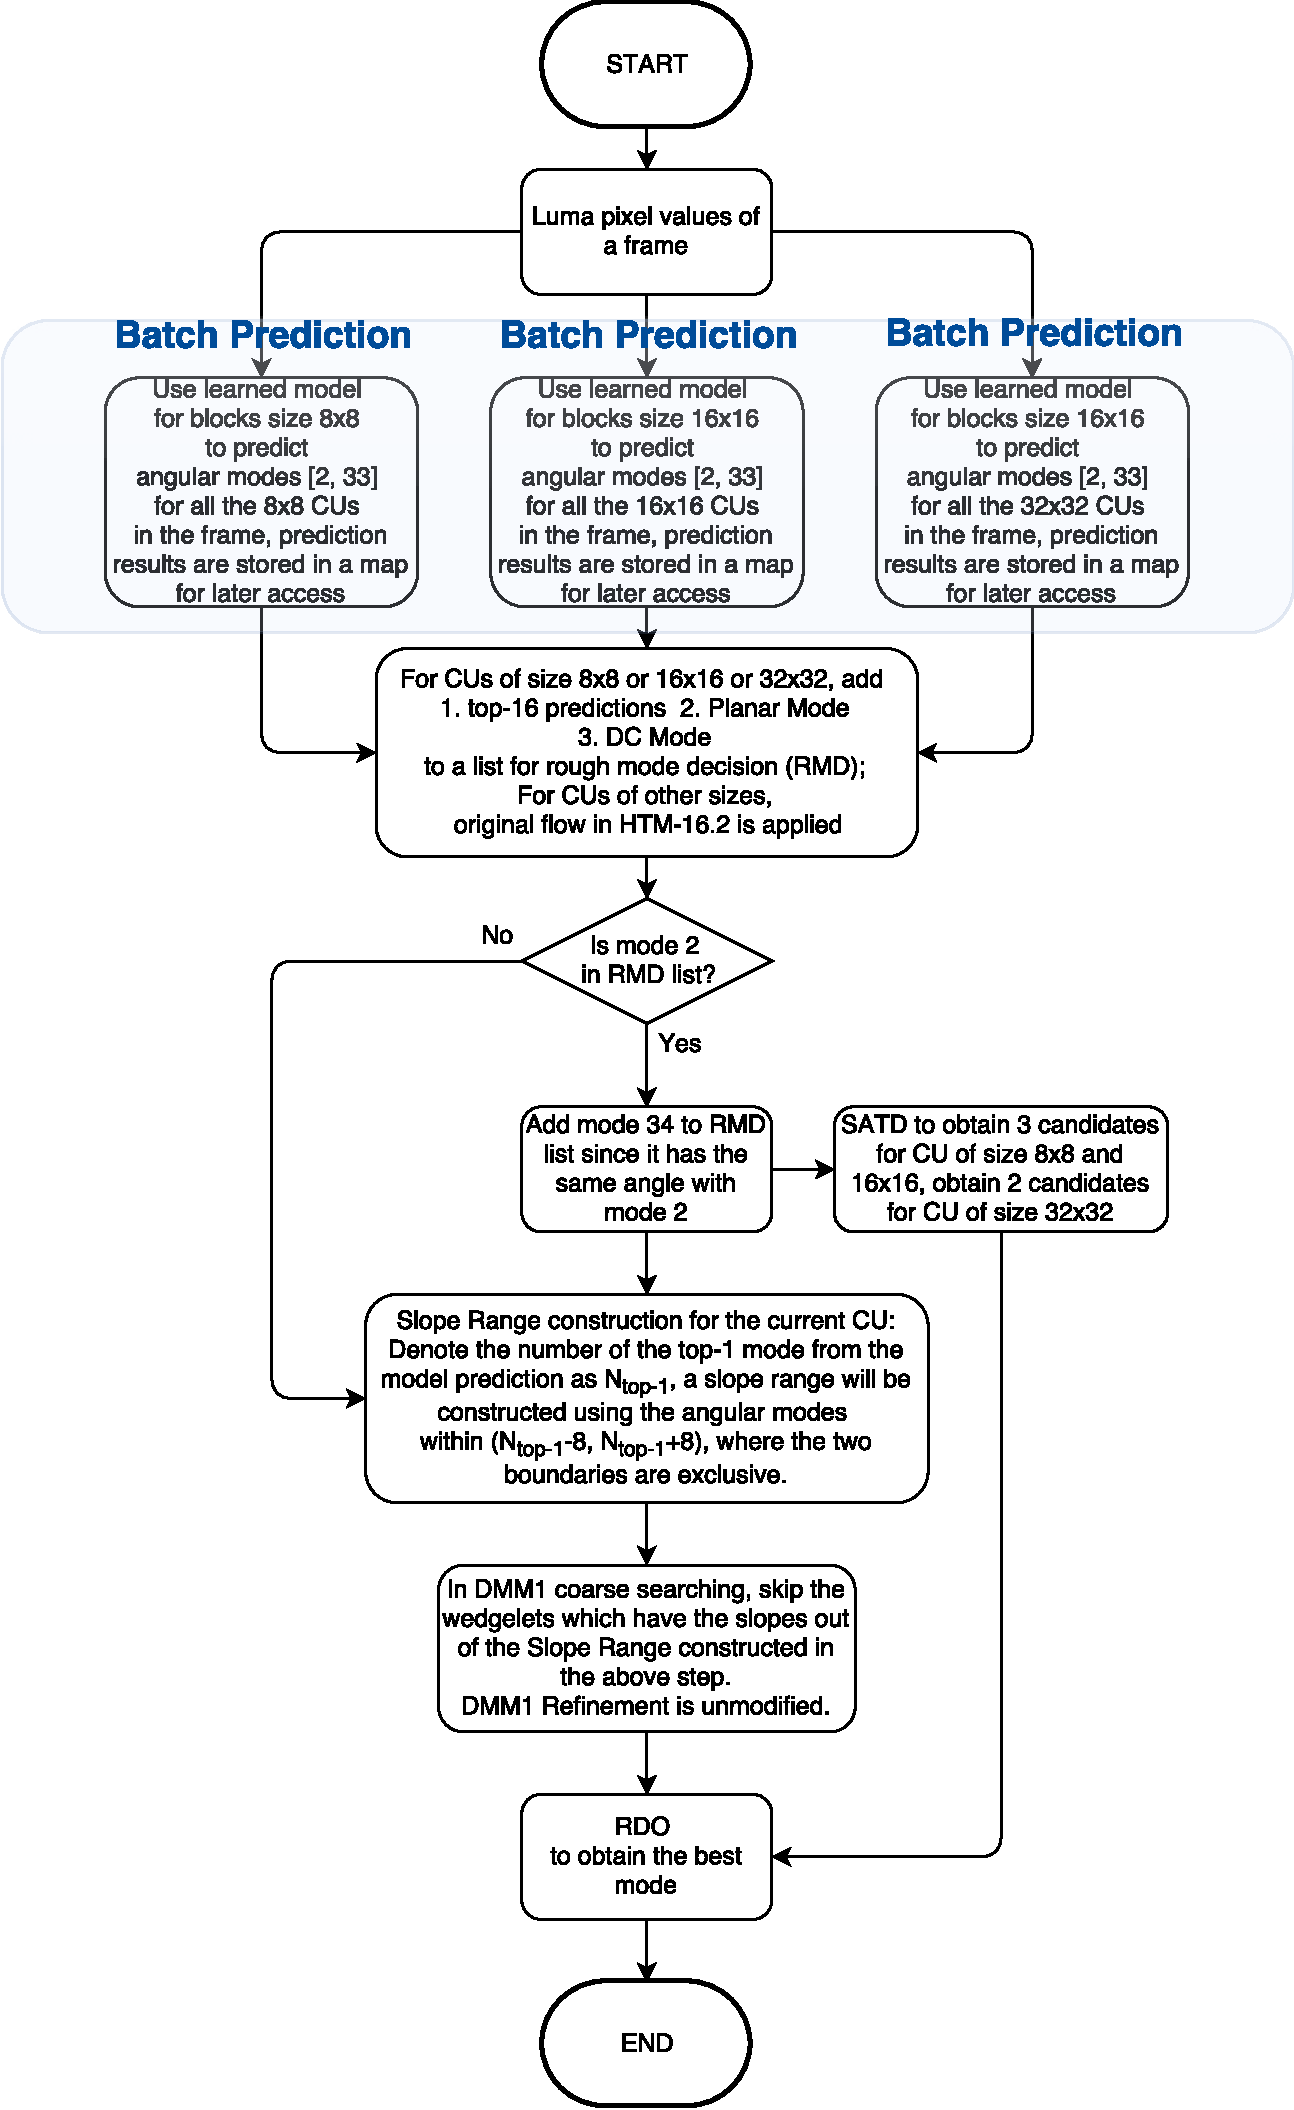
\includegraphics[height=0.92\textheight,keepaspectratio]{Figures/proposed-fast-depth-coding-algorithm}
    \caption[Flowchart for proposed fast depth coding 
    algorithm]{Flowchart for proposed fast depth coding 
    algorithm.}\label{fig:proposed-fast-depth-coding-algorithm}
\end{figure}

\section{Results of Experiments}\label{sec:simu-results}
The experiments are conducted on four video sequences shown in
Table~\ref{tab:data-for-experiments} 
% on page~\pageref{tab:data-for-experiments} 
to make sure every sample
that will be predicted has never been seen by the learned models.
Two metrics including \textbf{BD-BR} from~\parencite{RN234} and \textbf{BD-PSNR}
from~\parencite{RN235}
are used in the evaluations for the proposed fast 
depth coding algorithm.
\textbf{BD-BR} calculates the average difference between
Rate Distortion curves of two sets of synthesized views
where one set of views are synthesized from 
the reconstructed views from original encoder while 
the other set of views are synthesized from 
the reconstructed views from the encoder powered by
deep learning.
\textbf{BD-PSNR} is employed to assess the subjective 
quality of synthesized views.
The common test condition defined
in~\parencite{common-test-condition}
is used in our experiments.
All the frames from four video sequences in experiments 
are encoded as I-Frames.
\begin{table}[!htbp]
    \caption{Video sequences used for experiments}
    \bigskip\label{tab:data-for-experiments}
    \centering
    \begin{tabular}{c c c c c}
        \toprule
        \# & Name of the Sequence & Resolution & Usage & Number of Frames\\
        \midrule
        1 & Newspaper & \(1024\times768\) & Simulation & 300\\
        2 & GhostTownFly & \(1920\times1088\) & Simulation & 250\\
        3 & PoznanHall2 & \(1920\times1088\) & Simulation & 200\\
        4 & Shark & \(1920\times1088\) & Simulation & 300\\
        \bottomrule
    \end{tabular}
\end{table}

Table~\ref{tab:ts-dmm}
% on page~\pageref{tab:ts-dmm}
shows the time saving for DMM1 wedgelet searching process together 
with the coding performance.
Table~\ref{tab:ts-total}
% on page~\pageref{tab:ts-total}
presents the time saving for total encoding and the coding performance.

\begin{table}[!htbp]
    \caption{Time saving for wedgelet searching and coding performance of proposed method}
    \bigskip\label{tab:ts-dmm}
    \centering
    \begin{tabular}{c c c c c c c}
        \toprule
         & \multicolumn{4}{c}{Time saving for DMM1} & & \\\cline{2-5}
        Sequences & QP34 & QP39 & QP42 & QP45 & BD-BR & BD-PSNR \\
        \midrule
        Newspaper       & 63.76 & 64.94 & 71.98 & 74.14 & 0.98\% & -0.02dB \\
        PoznanHall2    & 71.08 & 71.08 & 66.36 & 71.27 & 1.64\% & -0.05dB \\
        GhostTownFly       & 62.00 & 56.20 & 51.60 & 58.87 & 0.65\% & -0.02dB \\
        Shark           & 63.55 & 58.66 & 63.26 & 63.34 & 1.04\% & -0.03dB \\
    \end{tabular}
\end{table}

\begin{table}[!htbp]
    % \begin{table}[!htbp]
    \caption{Time saving for total encoding and coding performance of proposed method}
    \bigskip\label{tab:ts-total}
    \centering
    % \resizebox{\textwidth}{!}
    % {
    \begin{tabular}{c c c c c c c}
        \toprule
         & \multicolumn{4}{c}{Time saving for total encoding} & & \\\cline{2-5}
        Sequences & QP34 & QP39 & QP42 & QP45 & BD-BR & BD-PSNR \\
        \midrule
        Newspaper       & 27.33 & 27.20 & 27.78 & 27.38 & 0.98\% & -0.02dB \\
        PoznanHall2     & 29.00 & 28.34 & 28.75 & 19.04 & 1.64\% & -0.05dB \\
        GhostTownFly    & 32.52 & 31.19 & 31.25 & 32.07 & 0.65\% & -0.02dB \\
        Shark           & 38.94 & 31.26 & 37.33 & 36.86 & 1.04\% & -0.03dB \\
    \end{tabular}
    % }
\end{table}

From the experimental statistics shown in the two tables above,
our fast depth coding algorithm achieves
an average time reduction of 64.6\% in wedgelet searching 
during 3D-HEVC encoding
while the BD performance only has a trivial decrease.
It is noticed that the values of \textbf{BD-PSNR} almost stayed
unchanged comparing
with the original implementation from the reference software
of 3D-HEVC\@.
The models trained by deep learning
were trying their best to keep the originality of the
pixel blocks that they have seen during the encoding process.
However, the learned models have no idea of how to
adjust their prediction results by taking the bitrate
into consideration.
For this reason, the perceptual visual qualities of the videos
are well preserved while the performance on bitrate
decreased a little as 
a penalty.
In each single encoding activity for a video sequence, 
the time saving percent for whole encoding process is lower than 
the time saving percent for DMM1 but still the overall results
achieved by the proposed fast depth coding algorithm
can be considered as excellent when
comparing with the original implementation of 3D-HEVC\@.
